%% Reliability-Targeted Bedtime Planning with Explicit Infeasibility
%% IEEE ICHI 2027 -- Early Bird track.
%%
%% Confirmed against the ICHI 2027 CFP, 2026-09-13:
%%   Deadline  21 Sep 2026 23:59 AoE  (= 22 Sep 11:59 UTC)
%%   Notify    14 Nov 2026 (intended)
%%   Limit     10 pages main paper, PLUS references (references are free)
%%   Review    double-blind; anonymise the manuscript AND blind any
%%             references, links or repositories revealing authorship
%%   Track     long papers only; OpenReview
%% https://ichi2027.github.io/ICHI2027/call-for-early-submission.html
%%
%% Build:  pdflatex ichi2027 && pdflatex ichi2027
%% Figures: regenerate with  python evaluation/run_study.py --figures figures/
%%          then copy figures/*.pdf into paper/figures/

\documentclass[conference]{IEEEtran}
\IEEEoverridecommandlockouts

\usepackage{cite}
\usepackage{amsmath,amssymb}
\usepackage{graphicx}
\usepackage{booktabs}
\usepackage{algorithm}
\usepackage{algpseudocode}
\usepackage{url}
\usepackage[T1]{fontenc}

\graphicspath{{figures/}}

% Tighter floats; the page budget is the binding constraint here.
\setlength{\textfloatsep}{8pt plus 2pt minus 2pt}
\setlength{\floatsep}{8pt plus 2pt minus 2pt}
\setlength{\intextsep}{8pt plus 2pt minus 2pt}

\begin{document}

\title{Reliability-Targeted Bedtime Planning\\with Explicit Infeasibility}

%% ---------------------------------------------------------------
%% DOUBLE-BLIND. Restore the real author block only for camera-ready.
%% ---------------------------------------------------------------
\author{\IEEEauthorblockN{Anonymous Authors}
\IEEEauthorblockA{Affiliation withheld for double-blind review}}

\maketitle

\begin{abstract}
Sleep applications forecast: given tonight's behaviour they predict an outcome.
A person with a fixed obligation the next morning has the inverse question,
which is a constraint rather than a prediction---\emph{what must I do tonight to
be up at 05:40?}---and existing systems answer it regardless of whether their
model supports an answer. We invert a trained sleep model against a required
reliability, partitioning inputs by what a person can change within the planning
horizon, and return an explicit infeasibility verdict with counterfactual
attribution when no admissible plan reaches the target. Validated against
exhaustive search over seven ground-truth models, the planner never promises an
unreachable target, returns the latest feasible bedtime in every case, and
selects a minimal set of changes; its failure mode is conservatism. On two
public wearable cohorts (85 participants, 5{,}432 person-nights) the underlying
models are weak: $R^2$ 0.186 for sleep duration on the larger cohort and
$-0.090$ on the smaller, where it fails to replicate, and AUC 0.660 for
wake-time regularity, which does replicate. What the models do have is
calibration (ECE 0.0148), which is what a refusal mechanism actually needs. We
also find that a physiologically-structured synthetic panel overstates
predictability by roughly fourfold in $R^2$, which we report because training
sleep models on simulated data is common. Weak models motivate rather than
undermine the contribution: a planner built on a signal this thin should decline
to promise, and we show which component makes that possible.
\end{abstract}

\begin{IEEEkeywords}
sleep, wearable sensing, algorithmic recourse, counterfactual explanation,
model inversion, calibration, health informatics
\end{IEEEkeywords}

%% ===============================================================
\section{Introduction}

Alarm and sleep applications are forecasters. Given a night's behaviour they
report a predicted duration, a sleep score, or a probability of waking well. The
user is left to interpret a number and infer a remedy.

A person with a hard obligation has a different question, and it is a
constraint: \emph{I must be up at 05:40 and I cannot miss it. What do I have to
do tonight?}

Forward prediction cannot answer this. Worse, it cannot decline to answer: a
system that reports a probability reports one whether or not its model supports
the inference, and a user who must not oversleep is exactly the user least well
served by unwarranted confidence.

We make three contributions.

\textbf{A planning formulation.} We treat a trained sleep-outcome model as a
constraint to solve against rather than a predictor to read, searching for the
latest bedtime meeting a required reliability. The objective is the least
behavioural cost satisfying the constraint, not the safest available plan.

\textbf{A partition by planning horizon.} Inputs divide into what a person can
change \emph{tonight}, what reflects accumulated habit and takes weeks, and what
is fixed. This is what makes a plan actionable, and---as our ablation
shows---it is also what keeps the planner from promising things nobody can do
before bed.

\textbf{Infeasibility as a first-class output.} When no admissible plan reaches
the target, the system says so, reports the achievable ceiling, and attributes
the shortfall to the specific habit responsible. We argue this matters most
exactly when models are weak, and we show on real data that models in this
domain are weak.

Section~\ref{sec:related} positions the work against counterfactual explanation
and algorithmic recourse, where the technical machinery is closest.
Section~\ref{sec:method} specifies the method. Section~\ref{sec:results} reports
results from simulation and two public cohorts. Sections~\ref{sec:limitations}
and~\ref{sec:conclusion} state what the evidence does not support.

%% ===============================================================
\section{Related Work}
\label{sec:related}

\subsection{Counterfactual explanation and algorithmic recourse}

The closest technical neighbours are counterfactual explanation~\cite{wachter}
and algorithmic recourse~\cite{ustun,dice}. Wachter et al.~\cite{wachter}
generate the minimal change to an input that would flip a model's decision;
DiCE~\cite{dice} extends this to diverse sets of such changes. Ustun et
al.~\cite{ustun} are nearest of all: they explicitly separate \emph{actionable}
inputs from \emph{immutable} ones and search only over the former, on the
grounds that recourse offered over age or marital status is no recourse at all.

We differ in three ways, and the third is the one we claim as novel.

\textbf{The constraint is a probability, not a label.} Recourse asks what flips
a decision already made about a person---loan denied, parole refused. We ask
what achieves a \emph{stated probability} of a future outcome the person chose
themselves. The search target is a continuous threshold on $f$, not a decision
boundary, and the objective is the least costly point satisfying it rather than
the nearest point across it.

\textbf{The partition is temporal, not binary.} Recourse divides inputs into
actionable and immutable. Sleep admits a third class that neither label fits:
sleep-timing consistency and habitual alarm response are entirely
changeable---over weeks. They are not immutable, but they are unavailable
\emph{tonight}. Treating them as actionable produces advice nobody can execute
before bed; treating them as immutable discards the most informative explanation
available when a target cannot be met. We therefore partition by planning
horizon rather than by mutability, and Section~\ref{sec:ablation} shows this is
the only component whose removal causes the planner to promise what cannot be
delivered.

\textbf{Infeasibility is an output, not a failure.} When no recourse exists,
recourse methods report that none was found. We treat that case as the primary
result: the system reports the achievable ceiling and attributes the shortfall
by counterfactual substitution over the habit partition, converting ``no plan
exists'' into ``the limit is not tonight, it is this habit, worth this much.''
For a user who must not oversleep, that is more actionable than a plan would be.

\subsection{Sleep prediction and smart alarms}

Smart alarms optimise \emph{when to ring within a window}, typically by
detecting a light sleep stage from movement or ambient sensing and triggering
inside it~\cite{smartalarm}. This is a different problem from ours: the window
is given and the system chooses a moment within it, whereas we take the wake
time as fixed and solve for the behaviour preceding it. It is also a problem
whose benefit is not settled---Campanella et al.~\cite{smartalarm} find little
overall effect of such a system on sleep inertia---which is part of why we
target the night before rather than the moment of waking.

Bedtime-reminder features in consumer platforms count back a fixed duration from
a target wake time, as do ``sleep cycle calculators'' that subtract multiples of
90 minutes. These are model-free rules; they cannot represent an individual's
response and, as Section~\ref{sec:refusal} shows, they have no mechanism for
recognising that a target is unreachable.

A substantial literature predicts sleep outcomes from wearable data, from deep
models of sleep quality~\cite{sathya} to next-night sleep duration in clinical
populations~\cite{fellger}. All of it runs forward: behaviour in, outcome out.
Our contribution is not a better predictor---ours is weak, and we report it as
such---but a way of using a predictor that stays honest when it is weak.

\subsection{Wearable sleep datasets}

We evaluate on LifeSnaps~\cite{lifesnaps} and PMData~\cite{pmdata}, both public
and both requiring no application. Neither records alarm interaction, which is
the central data limitation of this work: habitual snooze count and alarm
response latency are absent from every public wearable corpus we are aware of,
because no consumer device instruments the alarm itself.

Work on sleep-outcome prediction frequently trains on simulated panels when real
cohorts are unavailable. Section~\ref{sec:synthgap} quantifies what that costs
on this task.

%% ===============================================================
\section{Method}
\label{sec:method}

\subsection{Problem formulation}

Let $\mathbf{x} \in \mathbb{R}^d$ be a night's feature vector and
$f(\mathbf{x}) \rightarrow [0,1]$ a trained classifier estimating the
probability of waking on schedule. A forward system reports $f(\mathbf{x})$. We
instead solve, for a required reliability $\tau$: find the \textbf{latest}
bedtime $b$ such that $f(\mathbf{x}\ \text{with bedtime}\ b) \ge \tau$, and if
none exists, report that fact together with the achievable ceiling and its
cause.

\emph{Latest}, not earliest, is a design choice with a trade-off rather than an
obvious optimum. Among bedtimes satisfying the constraint, the latest imposes
the least behavioural cost, and a planner that always recommends the safest
available bedtime is needlessly punitive and will be ignored. But the latest
feasible bedtime is by construction the one with \textbf{no margin}: it sits
exactly at the constraint boundary, so any error in $f$ translates directly into
a missed wake. With the model accuracies reported in
Section~\ref{sec:synthgap}, that error is not small.

The objective is therefore exposed as a parameter---a deployment can require
$f \ge \tau + m$ for a margin $m$---and we make no claim that $m = 0$ is correct
for users. Which margin people actually want, and whether they trust a system
that cuts it fine, is a question for the deployment study of
Section~\ref{sec:limitations} rather than one this paper answers.

\subsection{Feature partition}

The $d$ inputs are partitioned into three classes, and only the first is
admissible in a same-night plan:

\begin{itemize}
\item \textbf{Controllable tonight}---bedtime, screen time before bed, caffeine,
      ambient noise, room temperature, stress, exercise.
\item \textbf{Habit-level}---sleep-timing consistency, habitual snooze count,
      habitual alarm response latency, accumulated sleep debt. Real determinants
      of wake reliability, but not changeable before tonight.
\item \textbf{Fixed}---age, chronotype, resting heart rate.
\end{itemize}

The partition is what makes a plan actionable. Section~\ref{sec:ablation} shows
it is also what keeps the planner sound: removing it is the only ablation that
produces promises the world cannot keep.

\subsection{Inverse planning}

\begin{algorithm}[t]
\caption{Bedtime sweep}
\label{alg:sweep}
\begin{algorithmic}[1]
\Require features $\mathbf{x}$, target $\tau$
\Ensure latest feasible bedtime or $\perp$, ceiling, full curve
\State $B \gets [26.00, 25.75, \dots, 20.00]$ \Comment{latest first, 0.25\,h}
\State $S \gets f_{\text{batch}}(\{\mathbf{x}\ \text{with bedtime}\ b : b \in B\})$
\State $\textit{best} \gets \max(S)$
\ForAll{$(b, s) \in \text{zip}(B, S)$}
  \If{$s \ge \tau$} \Return $b$, \textit{best}, curve \Comment{first hit is latest}
  \EndIf
\EndFor
\State \Return $\perp$, \textit{best}, curve
\end{algorithmic}
\end{algorithm}

\textbf{Algorithm~\ref{alg:sweep}.} The primary control is swept across its
admissible range [20:00, 02:00] at 15-minute resolution (25 candidates), scored
in one batched forward pass, and the latest candidate meeting $\tau$ is
returned.

Exhaustive scanning rather than gradient search is deliberate. A random forest's
response is a step function with no gradient to follow, the admissible range is
only 25 points wide, and the whole curve is worth returning for display.
Section~\ref{sec:sound} confirms the sweep returns the true latest feasible
bedtime in every simulated scenario including non-monotone response curves,
where a gradient method would settle in a local optimum.

\begin{algorithm}[t]
\caption{Greedy coordinate ascent}
\label{alg:ascent}
\begin{algorithmic}[1]
\Require features $\mathbf{x}$, target $\tau$, budget $R$
\Ensure modified features, achieved reliability, list of changes
\State $c \gets \mathbf{x}$;\ \ $r \gets f(c)$;\ \ \textit{steps} $\gets [\,]$
\For{$R$ rounds}
  \If{$r \ge \tau$} \textbf{break} \EndIf
  \State $M \gets \{\text{clamp}(v + \text{dir}\cdot\text{step}\cdot 3)\}$ per lever
  \State $M \gets \{m \in M : m\ \text{changes the current value}\}$
  \If{$M = \emptyset$} \textbf{break} \EndIf
  \State $G \gets f_{\text{batch}}(\{c \oplus m : m \in M\})$
  \State $i \gets \arg\max(G)$;\ \ \textit{gain} $\gets G[i] - r$
  \If{\textit{gain} $\le 0.002$} \textbf{break} \EndIf
  \State merge $M[i]$ into \textit{steps} \Comment{fold repeats on one lever}
  \State $c \gets c \oplus M[i]$;\ \ $r \gets G[i]$
\EndFor
\State \Return $c$, $f(c)$, \textit{steps}
\end{algorithmic}
\end{algorithm}

\textbf{Algorithm~\ref{alg:ascent}.} When bedtime alone is insufficient, the
remaining controllable inputs are searched one at a time. Two details matter for
reimplementation. \textbf{Re-scoring after each committed move} is what prevents
double-counting redundant levers: two levers acting through one physiological
channel do not contribute additively, and scoring them independently overstates
the plan. \textbf{Stopping as soon as $\tau$ is met} yields the fewest changes
that suffice rather than every change available;
Section~\ref{sec:sound} confirms the resulting set is exactly minimal.

$R = 8$. It was 3 until simulation showed the search exhausting its budget
rather than its options---a traced case reached 0.66 against a 0.70 target and
needed one further round. Raising it cut false refusals from 10 to 3 of 42 and
never once produced an unkeepable promise.

\subsection{Parameters}

Table~\ref{tab:levers} gives everything an implementation needs. Each lever has
a direction (the sign of the change expected to help), an admissible range, and
a step size; one round of Algorithm~\ref{alg:ascent} moves the chosen lever by
three steps. Room temperature is the one lever with no monotone direction: its
candidate is the set-point 20.5\,\textdegree C rather than an extreme, since
both hotter and colder are worse.

\begin{table}[t]
\caption{Controllable levers, and thresholds governing the search}
\label{tab:levers}
\centering
\small
\begin{tabular}{lccc}
\toprule
Lever & Dir. & Range & Step \\
\midrule
\texttt{bedtime\_hour}               & $-$ & 20.0--26.0\,h & 0.25 \\
\texttt{screen\_minutes\_before\_bed}& $-$ & 0--180\,min & 15 \\
\texttt{caffeine\_mg}                & $-$ & 0--400\,mg & 40 \\
\texttt{ambient\_noise\_db}          & $-$ & 20--70\,dB & 5 \\
\texttt{room\_temp\_c}       & set-pt. & 14--30\,\textdegree C & $\rightarrow$ 20.5 \\
\texttt{stress\_level}               & $-$ & 0--100 & 10 \\
\texttt{exercise\_minutes}           & $+$ & 0--120\,min & 20 \\
\midrule
\multicolumn{4}{l}{\emph{Habit feature $\rightarrow$ healthy reference (attribution)}}\\
\texttt{sleep\_consistency} & \multicolumn{3}{c}{85 / 100} \\
\texttt{snooze\_count}      & \multicolumn{3}{c}{0} \\
\texttt{alarm\_response\_ms}& \multicolumn{3}{c}{5{,}000\,ms} \\
\texttt{sleep\_debt\_hours} & \multicolumn{3}{c}{0} \\
\midrule
\multicolumn{4}{l}{\emph{Thresholds}}\\
Coordinate-ascent budget $R$   & \multicolumn{3}{c}{8 rounds} \\
Min.\ gain to commit a move    & \multicolumn{3}{c}{0.002} \\
Min.\ gain to report a lever   & \multicolumn{3}{c}{0.001} \\
Min.\ gain to report a habit cause & \multicolumn{3}{c}{0.01} \\
Bedtime resolution             & \multicolumn{3}{c}{0.25\,h over 20:00--02:00} \\
\bottomrule
\end{tabular}
\end{table}

Two distinct trailing windows govern the derived features, a point easily
missed. \textbf{Habit features use a 7-night window}:
\texttt{sleep\_consistency} is the standard deviation of night-anchored bedtime
over the preceding 7 nights, mapped linearly onto 0--100 with an SD of 3\,h
scoring zero; \texttt{sleep\_debt\_hours} is the cumulative shortfall against an
assumed 8\,h need over the same window, clipped to $[-2, 4]$. \textbf{The
wake-proxy baseline uses a 28-night window}, minimum 3 observations in the
(participant, day-type) bucket. \texttt{chronotype\_code} bins each
participant's median night-anchored bedtime: lark below 23:00, intermediate to
24:30, owl beyond. Night-anchored hour maps clock time onto a 20--26 axis so a
night spanning midnight does not wrap, splitting at 12:00.

\subsection{Infeasibility and attribution}

If neither algorithm reaches $\tau$, the planner does not return a bedtime. It
returns the achievable ceiling and attributes the shortfall to the
\textbf{habit} partition by counterfactual substitution: each habit feature is
independently set to a healthy reference value and re-scored, and those yielding
a gain above 0.01 are reported, ranked, with a weeks-not-tonight horizon.

The output is therefore of the form \emph{``95\% is not reachable tonight; the
best available combination reaches 60\%. What limits you is habit rather than
tonight: responding to your alarm on the first attempt is worth 30 points on its
own. Set a backup alarm on a second device.''} Fig.~\ref{fig:search} contrasts
the two cases the planner distinguishes.

\begin{figure}[t]
\centering
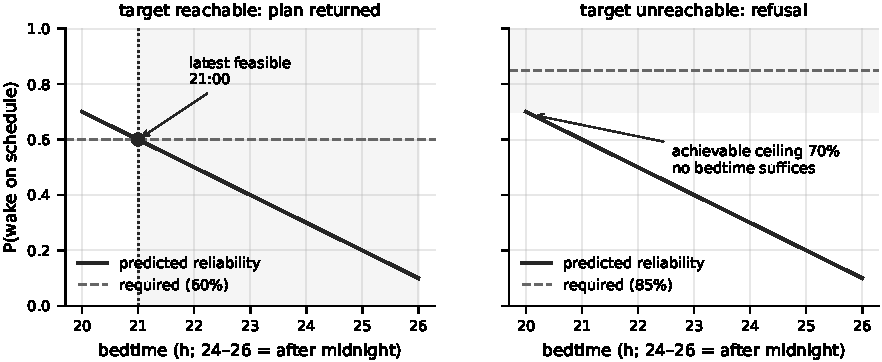
\includegraphics[width=\columnwidth]{fig1_inverse_search.pdf}
\caption{Inverse search on a feasible night (left) and an infeasible one
(right). The sweep returns the latest bedtime clearing $\tau$; where the whole
curve sits below $\tau$, the planner refuses and reports the ceiling instead of
a bedtime.}
\label{fig:search}
\end{figure}

\subsection{Datasets}

Two public wearable cohorts, both downloadable without application
(Table~\ref{tab:data}). Sleep timing in LifeSnaps exists only in a 9.7\,GB
MongoDB dump; the released CSVs contain none. Nights carrying several sleep
episodes are folded to the longest, giving one row per participant-night.

\begin{table}[t]
\caption{Cohorts}
\label{tab:data}
\centering
\small
\begin{tabular}{lcc}
\toprule
 & LifeSnaps~\cite{lifesnaps} & PMData~\cite{pmdata} \\
\midrule
Participants with sleep data & 69 & 16 \\
Person-nights & 3{,}551 & 1{,}881 \\
Duration & $\sim$4 months & 5 months \\
Device & Fitbit Sense & Fitbit Versa 2 \\
Licence & CC BY 4.0 & see source \\
\bottomrule
\end{tabular}
\end{table}

\textbf{Feature availability is the binding constraint.} Of the 15 model inputs,
3--4 are directly available, 5 derivable under stated assumptions, and 6--7
absent entirely. Critically, \textbf{no public wearable dataset records alarm
interaction}, so habitual snooze count and alarm response latency---half the
habit partition---cannot be populated. Of the seven controllable levers, only
bedtime, stress and exercise exist.

\subsection{Target construction}

Neither dataset contains an alarm, so the outcome must be constructed. We label
a night successful when the participant woke no more than $N$ minutes after
their habitual wake time for that kind of day, with $N = 30$. Three choices,
each defensible and each reported with a sensitivity analysis:

\begin{enumerate}
\item \textbf{One-sided.} Oversleeping is waking \emph{late}. A symmetric window
      scores someone who woke forty minutes early as a failure, which is a
      different construct.
\item \textbf{Day-type aware.} People wake later at weekends by choice. Against
      a pooled baseline the label degenerates into a weekday detector.
\item \textbf{Baseline from prior nights only}, over a 28-night window with at
      least three observations, computed within (participant, day-type) with
      \textbf{no fallback to pooled history}. Borrowing pooled history for a
      thin weekend bucket judges a 10:00 lie-in against a 07:00 weekday habit
      and scores three hours of oversleeping---reintroducing exactly the
      contamination the bucketing removes. This costs ${\sim}11\%$ of nights and
      is the cheaper error.
\end{enumerate}

\textbf{We call this wake-time regularity, not wake success.}
Section~\ref{sec:limitations} explains why.

\subsection{Models and protocol}

Random forests (200 trees, depth 12, minimum leaf 8, seed 42) for both the
duration regressor and the regularity classifier, identical to the configuration
used on the synthetic panel so that differences isolate the data.

\textbf{Splits are by participant.} A participant contributes ${\sim}50$ nights;
splitting rows at random lets a model identify the person rather than learn
anything about nights. All reported figures are means over 8 grouped splits.

\textbf{Outcome columns are never predictors.} Sleep duration is approximately
time-in-bed $\times$ efficiency, so time-in-bed, efficiency and wake time are
excluded by an assertion rather than by convention. For the regularity
classifier, sleep duration is additionally excluded: combined with bedtime it
reconstructs wake time and hence the label.

\textbf{Habit features use strictly prior nights.} Including tonight's own value
in its trailing window leaks the target into the predictors.

\textbf{Uncertainty is clustered.} All intervals come from resampling
participants, never rows. Mixed-effects models (random intercept; GEE with
exchangeable working correlation for the binary outcome) account for repeated
nights.

%% ===============================================================
\section{Results}
\label{sec:results}

\subsection{Synthetic data substantially overstates predictability}
\label{sec:synthgap}

Retrained on real cohorts with identical model, features and protocol
(Table~\ref{tab:synthgap}, Fig.~\ref{fig:synthgap}), $R^2$ falls by roughly a
factor of four. Across splits it ranges $-0.077$ to $+0.395$, so no single-split
figure is reportable; the interval nonetheless excludes zero, so the model does
beat the mean on LifeSnaps.

\begin{table}[t]
\caption{Sleep-duration regression across cohorts}
\label{tab:synthgap}
\centering
\small
\begin{tabular}{lccc}
\toprule
Cohort & MAE (h) & $R^2$ & vs.\ mean \\
\midrule
Synthetic panel & 0.403 & $\mathbf{+0.702}$ & $+45.6\%$ \\
LifeSnaps & 1.016 & $\mathbf{+0.186}$ \footnotesize{(CI 0.075--0.297)} & $+15.0\%$ \\
PMData & 1.072 & $\mathbf{-0.090}$ & $+3\%$ \\
\bottomrule
\end{tabular}
\end{table}

\begin{figure}[t]
\centering
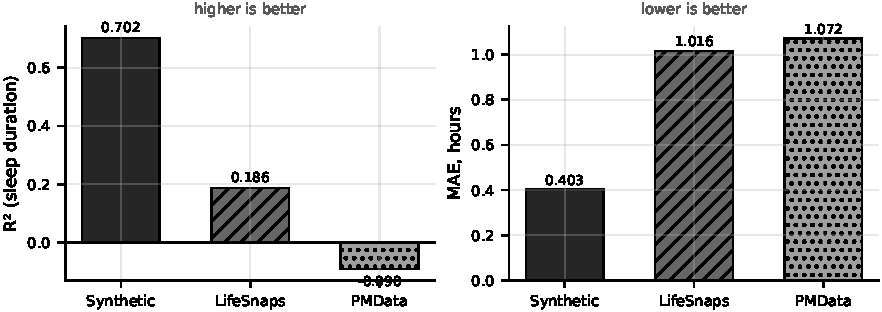
\includegraphics[width=\columnwidth]{fig2_synthetic_vs_real.pdf}
\caption{The synthetic-to-real gap. Identical model, features and protocol; only
the data changes.}
\label{fig:synthgap}
\end{figure}

\textbf{On PMData the duration model does not replicate.} $R^2 = -0.090$ is
worse than predicting the mean, and we state that as a failed replication rather
than as a smaller effect. The cohort is 16 participants and the interval is
correspondingly wide, but the result is what it is, and a reader should treat
the duration model as supported by one cohort rather than two.

The regularity model does replicate: AUC 0.761 synthetic against 0.660 (95\% CI
0.610--0.710) on LifeSnaps and 0.675 on PMData---marginally \emph{higher} on the
second cohort. Both intervals exclude chance. Unweighted accuracy exceeds the
majority-class baseline by only 1.0 point, so the discrimination is real but
slight.

An oracle predicting each held-out participant's own mean duration beats the
model in 5 of 8 splits. Consistent with this, the unconditional intraclass
correlation is \textbf{0.336} for sleep duration---a third of the variance is a
stable person-level trait---but only \textbf{0.060} for wake regularity, which
is almost entirely night-to-night.

Two predictors survive in both models under different estimators: later bedtime
($-0.295$ SD of sleep duration, CI $-0.354$ to $-0.236$; OR 0.677, CI
0.496--0.925 for regularity) and resting heart rate. \textbf{No habit feature
reaches significance in either model.}

\subsection{The stated reliability is calibrated}

Over 3{,}180 held-out person-nights from 46 participants
(Table~\ref{tab:calib}), \textbf{ECE is 0.0148 (95\% CI 0.0139--0.0571)}. The
interval is wide and right-skewed; the point estimate alone overstates the
precision.

\begin{table}[t]
\caption{Reliability diagram, binned}
\label{tab:calib}
\centering
\small
\begin{tabular}{ccc}
\toprule
Predicted & $n$ & Observed \\
\midrule
0.66 & 436 & 0.649 \\
0.76 & 1{,}115 & 0.765 \\
0.84 & 1{,}178 & 0.832 \\
0.93 & 127 & 0.929 \\
\bottomrule
\end{tabular}
\end{table}

Calibration alone is insufficient, and we report Brier alongside for that
reason: a predictor that always returns the base rate achieves a \emph{perfect}
ECE of 0.0000 while carrying no information. Brier separates them---0.1727 (CI
0.1490--0.2003) against 0.1898 for the base-rate predictor. The honest
description is \textbf{well calibrated, weakly informative}, which is the
combination honest refusal requires: the model does not know much, but it knows
how much it knows.

\textbf{What this result does and does not claim.} Calibration is measured
against the constructed target of Section~\ref{sec:method}, and
Section~\ref{sec:limitations} reports that this target has no detectable
association with how participants said they felt. The two statements are
compatible, and the distinction matters enough to make explicit: this is a claim
about \textbf{internal consistency}, not about external validity. When the
system states 85\%, roughly 85\% of those nights satisfy the stated criterion.

That is precisely the property a refusal mechanism requires, because refusal is
a statement about the model's own confidence rather than about the world: a
system declining to promise 95\% is asserting that its own estimate does not
reach 95\%, and that assertion is only meaningful if its estimates mean what
they say. It is \emph{not} a claim that waking within 30 minutes of one's
habitual time is a valuable outcome. Establishing that the criterion is worth
caring about requires the deployment study this paper does not have.

\subsection{The algorithm is sound but incomplete}
\label{sec:sound}

The recommendation cannot be validated observationally---it is conditional on a
bedtime no participant adopted on our instruction. We therefore validate the
\emph{algorithm} against exhaustive search over seven analytic ground-truth
models $\times$ six targets, including non-monotone response curves, redundant
levers, interacting levers and hard ceilings (Table~\ref{tab:sound}).

\begin{table}[t]
\caption{Algorithmic validation against exhaustive search}
\label{tab:sound}
\centering
\small
\begin{tabular}{lc}
\toprule
Property & Result \\
\midrule
Sweep returns the latest feasible bedtime & $\mathbf{42/42}$ \\
Promises only reachable targets (soundness) & \textbf{0 violations} \\
Lever set exactly minimal when successful & 100\% \\
Refuses only unreachable targets (completeness) & 92.9\% (3/42) \\
\bottomrule
\end{tabular}
\end{table}

The planner never over-promises at any iteration budget tested. Its failure mode
is conservatism---refusing some achievable targets---which for a system whose
contribution is honest refusal is the correct direction to err. Behaviour at the
achievable ceiling is exact: a target equal to the ceiling is promised, one
0.001 above is refused.

\subsection{Refusal beats promising, and forward prediction refuses best}
\label{sec:refusal}

Table~\ref{tab:refusal} reports over-promise rate---promising a target the
held-out participant's own achieved rate could not deliver. At a 0.95 target the
model-free planners promise every night and are wrong every time
(Fig.~\ref{fig:refusal}). That comparison is real but weak: neither has any mechanism for declining, so
measuring their over-promise rate largely measures that absence. We report it
because it is the behaviour deployed systems actually exhibit, not because it is
a demanding baseline.

\begin{table}[t]
\caption{Over-promise rate by planner and target (lower is better)}
\label{tab:refusal}
\centering
\small
\begin{tabular}{lcccc}
\toprule
Target & Always & 90-min & Inverse & Forward \\
 & promise & rule & planner & prediction \\
\midrule
0.70 & 0.376 & 0.376 & 0.372 & \textbf{0.294} \\
0.80 & 0.614 & 0.614 & 0.473 & \textbf{0.261} \\
0.90 & 0.867 & 0.867 & 0.068 & \textbf{0.016} \\
0.95 & 1.000 & 1.000 & 0.040 & \textbf{0.013} \\
\bottomrule
\end{tabular}
\end{table}

\begin{figure}[t]
\centering
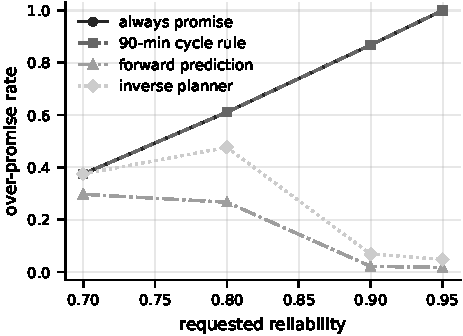
\includegraphics[width=\columnwidth]{fig4_refusal_quality.pdf}
\caption{Over-promise rate against target reliability. Model-free planners
diverge as the target rises because they cannot decline.}
\label{fig:refusal}
\end{figure}

\textbf{The informative comparison is forward prediction}, which uses the same
model and differs only in that it does not search---and it beats the inverse
planner at every target. We report this rather than omitting it, and we do not
count it in our favour, but it should not be read as evidence that inversion
hurts. The two make different kinds of promise. Forward prediction claims
\emph{tonight, as it already stands, clears the target}, and the observed night
tests that claim directly. Inversion claims \emph{a different bedtime would
clear it}, and no participant adopted a different bedtime on our instruction.
The observed outcome therefore tests a night the recommendation was not about.

This is the counterfactual gap of Section~\ref{sec:sound} appearing in the data
rather than in the argument: the comparison is between a claim this dataset can
check and one it cannot. Separating them requires intervention, not more
observation.

\subsection{Every component contributes differently}
\label{sec:ablation}

\begin{table}[t]
\caption{Ablations. Only removing the habit partition breaks soundness.}
\label{tab:ablation}
\centering
\small
\begin{tabular}{lcccc}
\toprule
Ablation & Verdict & False & Broken & Bedtime \\
 & correct & refusals & promises & optimal \\
\midrule
Full planner & 0.929 & 3 & \textbf{0} & 1.00 \\
No bedtime sweep & 0.881 & 5 & 0 & \textbf{0.69} \\
No coordinate ascent & \textbf{0.762} & \textbf{10} & 0 & 1.00 \\
No habit partition & 0.857 & 3 & \textbf{3} & 1.00 \\
No attribution & 0.929 & 3 & 0 & 1.00 \\
\bottomrule
\end{tabular}
\end{table}

The sweep buys optimality rather than feasibility: without it, minimality falls
from 1.00 to 0.56 and the planner recommends earlier bedtimes than necessary
(Table~\ref{tab:ablation}, Fig.~\ref{fig:ablation}). Coordinate ascent buys
completeness. \textbf{The habit partition is the only component whose removal
breaks soundness}---without it the planner offers plans requiring changes nobody
can make before bed. The attribution changes no verdict at all; what it changes
is whether the user is told why (2 habit causes named versus 0).

\begin{figure}[t]
\centering
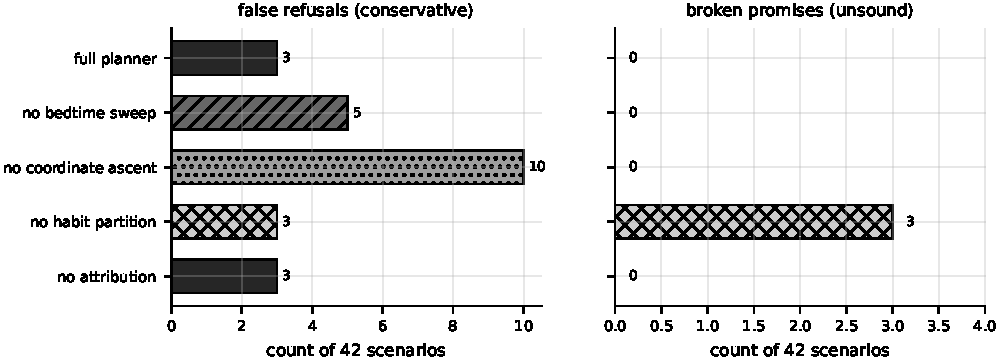
\includegraphics[width=\columnwidth]{fig5_ablation.pdf}
\caption{Removing each component. Broken promises appear only when the habit
partition is removed.}
\label{fig:ablation}
\end{figure}

\textbf{This result is the paper's strongest claim and its least externally
grounded, and the two facts are connected.} The partition is what the ablation
identifies as load-bearing, yet it is exercised here only in simulation, and two
of its four inputs---habitual snooze count and alarm response latency---exist in
no public wearable dataset, so no observational analysis in this paper can test
it. The component we claim matters most is therefore demonstrated entirely
within a world we specified. We take the simulation as evidence that the
mechanism works as designed, not as evidence that it is calibrated to human
sleep; only instrumented alarm data can supply the latter.

\subsection{Observational evidence is directionally positive but inconclusive}

Table~\ref{tab:matched} compares nights where a participant coincidentally slept
near the recommended hour against their own other nights. The direction is
positive at every tolerance and no interval excludes zero. With 9--11
participants contributing a paired difference this is underpowered by
construction, and we report it as suggestive only. Detecting an effect of the
observed magnitude would require approximately \textbf{50--75 participants}.

\begin{table}[t]
\caption{Within-participant matched comparison}
\label{tab:matched}
\centering
\small
\begin{tabular}{lcccc}
\toprule
Tol. & Matched & Particip. & Diff. & 95\% CI \\
\midrule
$\pm$15\,min & 43 & 9 & $+0.085$ & $-0.055$--$+0.225$ \\
$\pm$30\,min & 86 & 9 & $+0.045$ & $-0.128$--$+0.217$ \\
$\pm$45\,min & 137 & 11 & $+0.093$ & $-0.043$--$+0.230$ \\
$\pm$60\,min & 168 & 11 & $+0.071$ & $-0.056$--$+0.199$ \\
\bottomrule
\end{tabular}
\end{table}

%% ===============================================================
\section{Limitations}
\label{sec:limitations}

We state these before a reader has to find them.

\textbf{The target is constructed, not measured.} Neither dataset contains an
alarm, an intended wake time, or any record of whether a participant had
somewhere to be. Our label measures deviation from personal schedule and nothing
more.

\textbf{The target showed no association with wellbeing.} Tested against
PMData's daily self-reported sleep quality ($d = -0.093$), readiness ($-0.026$)
and LifeSnaps' tiredness indicator ($-0.041$), all effects were negligible and
two pointed the wrong way. Restricting to weekdays did not help. The plain
reading is that waking later than habit is usually a lie-in rather than a
failure. \textbf{We therefore renamed the target from wake success to wake-time
regularity}, and the paper claims nothing about how anyone felt.

\textbf{The models are weak in absolute terms.} $R^2$ 0.186 and AUC 0.660
explain a minority of variance. We argue this motivates rather than undermines
the contribution---a planner built on a signal this thin \emph{should} decline
to promise---but a reader who wants strong point predictions will not find them.

\textbf{The system was developed against synthetic data, and that development
was optimistic.} The planner and its thresholds were built and tuned on a
physiologically-structured simulated panel that we now know overstates
predictability by roughly a factor of four in $R^2$ and 0.10 in AUC. We report
the gap as a finding in Section~\ref{sec:synthgap} because training sleep models
on simulated panels is common practice, but it is also a limitation of this work
specifically: design decisions made against the simulation may be tuned to a
world more predictable than the real one. The parameters in
Table~\ref{tab:levers} were re-examined against real data and simulation ground
truth, and one---the coordinate-ascent budget---was changed as a result; we
cannot rule out that others carry the same bias.

\textbf{Half the habit partition is unpopulated.} Habitual snooze count and
alarm response latency are absent from every public wearable dataset, because no
consumer device instruments the alarm. The infeasibility attribution therefore
runs on two of its four intended inputs.

\textbf{Four of seven controllable levers are absent.} Only bedtime, stress and
exercise exist in these cohorts. The coordinate-ascent results in
Section~\ref{sec:ablation} are measured in simulation with the full lever set
and are therefore an upper bound on what that component contributes in
deployment today.

\textbf{The simulation scenarios are ours.} Soundness holds across seven
ground-truth models we designed, including cases built to defeat greedy search.
They are principled rather than convenient, but they are not a proof, and a
different family of response surfaces might expose different behaviour.

\textbf{No deployment study.} The end-to-end claim---that following the advice
improves waking---is not established and cannot be from retrospective data. Our
matched-subset analysis is directionally positive and underpowered. Establishing
it requires giving people the recommendation and measuring what follows.

\textbf{Cohort generalisability.} 85 participants across two cohorts, neither
demographically representative. Neither dataset yields a numeric age (LifeSnaps
de-identifies to $<$30/$\ge$30; PMData ships no demographics), so no
age-adjusted analysis is possible.

\textbf{Sleep staging is consumer-grade.} Fitbit's sleep classification is not
polysomnography, and its error is not independent of the behaviours we model.

%% ===============================================================
\section{Conclusion}
\label{sec:conclusion}

We treated a sleep model as a constraint rather than a forecast, and asked what
a person must do tonight to reach a wake time at a reliability they choose.
Three things follow from that change of question. Inputs must be partitioned by
what is changeable within the planning horizon, and that partition is not the
actionable/immutable split used in algorithmic recourse---sleep's most
informative levers are changeable over weeks and unavailable tonight. The search
must be validated against something, and since no observational cohort contains
the counterfactual, we validated against exhaustive search over ground-truth
models built to defeat it: the planner never promised a target it could not
reach, returned the latest feasible bedtime in every case, and erred only by
refusing three times when a plan existed. And infeasibility must be reported
rather than suppressed, because the underlying models are weak---$R^2$ 0.186 and
AUC 0.660 on real cohorts, against the fourfold-inflated $R^2$ a synthetic panel
reports for the same task.

The weakness is the argument, not an embarrassment beside it. A planner with
this much signal should decline to promise, and our ablation identifies the
horizon partition as the single component whose removal makes it promise what
cannot be delivered. What we have not shown is that following the advice
improves waking; that requires giving people the recommendation and measuring
what happens, and our matched-subset analysis is only large enough to size that
study at 50--75 participants. The method is ready for it. The claim is not yet
earned.

\section*{Reproducibility}

All results regenerate from committed code, with pinned versions and fixed
seeds; 311 tests cover the pipeline, including assertions that participant
splits are disjoint, that outcome columns cannot become predictors, and that
habit features use strictly prior nights. Datasets are not redistributed; both
are obtainable without application from the sources in
Table~\ref{tab:data}. Code and reproduction instructions are available at an
anonymised URL for review.\footnote{Anonymised artifact link to be inserted
before submission.}

%% ===============================================================
\begin{thebibliography}{9}

\bibitem{wachter}
S. Wachter, B. Mittelstadt, and C. Russell, ``Counterfactual explanations
without opening the black box: automated decisions and the GDPR,''
\emph{Harvard Journal of Law \& Technology}, vol.~31, no.~2, pp.~841--887, 2018.

\bibitem{ustun}
B. Ustun, A. Spangher, and Y. Liu, ``Actionable recourse in linear
classification,'' in \emph{Proc. Conf. Fairness, Accountability, and
Transparency (FAT*)}, 2019, pp.~10--19.

\bibitem{dice}
R. K. Mothilal, A. Sharma, and C. Tan, ``Explaining machine learning classifiers
through diverse counterfactual explanations,'' in \emph{Proc. Conf. Fairness,
Accountability, and Transparency (FAT*)}, 2020, pp.~607--617.

\bibitem{smartalarm}
C. Campanella, K. Byun, A. Senerat, L. Li, R. Zhang, S. Aristizabal, P. Porter,
and B. Bauer, ``The efficacy of a multimodal bedroom-based `smart' alarm system
on mitigating the effects of sleep inertia,'' \emph{Clocks \& Sleep}, vol.~6,
no.~1, pp.~183--199, 2024.

\bibitem{sathya}
A. Sathyanarayana, S. Joty, L. Fernandez-Luque, F. Ofli, J. Srivastava,
A. Elmagarmid, T. Arora, and S. Taheri, ``Sleep quality prediction from wearable
data using deep learning,'' \emph{JMIR mHealth and uHealth}, vol.~4, no.~4,
art.~e125, 2016.

\bibitem{fellger}
A. Fellger, G. Sprint, D. Weeks, E. Crooks, and D. J. Cook, ``Wearable
device-independent next day activity and next night sleep prediction for
rehabilitation populations,'' \emph{IEEE Journal of Translational Engineering in
Health and Medicine}, vol.~8, art.~2700509, 2020.

\bibitem{lifesnaps}
S. Yfantidou, C. Karagianni, S. Efstathiou, A. Vakali, J. Palotti, D. P.
Giakatos, T. Marchioro, A. Kazlouski, E. Ferrari, and
\v{S}. Girdzijauskas, ``LifeSnaps, a 4-month multi-modal dataset capturing
unobtrusive snapshots of our lives in the wild,'' \emph{Scientific Data},
vol.~9, art.~663, 2022.

\bibitem{pmdata}
V. Thambawita, S. A. Hicks, H. Borgli, H. K. Stensland, D. Jha, \emph{et al.},
``PMData: a sports logging dataset,'' in \emph{Proc. 11th ACM Multimedia Systems
Conf.\ (MMSys)}, 2020, pp.~231--236.

\end{thebibliography}

\end{document}
